% Options for packages loaded elsewhere
\PassOptionsToPackage{unicode}{hyperref}
\PassOptionsToPackage{hyphens}{url}
%
\documentclass[
]{article}
\usepackage{lmodern}
\usepackage{amssymb,amsmath}
\usepackage{ifxetex,ifluatex}
\ifnum 0\ifxetex 1\fi\ifluatex 1\fi=0 % if pdftex
  \usepackage[T1]{fontenc}
  \usepackage[utf8]{inputenc}
  \usepackage{textcomp} % provide euro and other symbols
\else % if luatex or xetex
  \usepackage{unicode-math}
  \defaultfontfeatures{Scale=MatchLowercase}
  \defaultfontfeatures[\rmfamily]{Ligatures=TeX,Scale=1}
\fi
% Use upquote if available, for straight quotes in verbatim environments
\IfFileExists{upquote.sty}{\usepackage{upquote}}{}
\IfFileExists{microtype.sty}{% use microtype if available
  \usepackage[]{microtype}
  \UseMicrotypeSet[protrusion]{basicmath} % disable protrusion for tt fonts
}{}
\makeatletter
\@ifundefined{KOMAClassName}{% if non-KOMA class
  \IfFileExists{parskip.sty}{%
    \usepackage{parskip}
  }{% else
    \setlength{\parindent}{0pt}
    \setlength{\parskip}{6pt plus 2pt minus 1pt}}
}{% if KOMA class
  \KOMAoptions{parskip=half}}
\makeatother
\usepackage{xcolor}
\IfFileExists{xurl.sty}{\usepackage{xurl}}{} % add URL line breaks if available
\IfFileExists{bookmark.sty}{\usepackage{bookmark}}{\usepackage{hyperref}}
\hypersetup{
  pdftitle={STAT 33B Homework 2},
  pdfauthor={Ming Fong (3035619833)},
  hidelinks,
  pdfcreator={LaTeX via pandoc}}
\urlstyle{same} % disable monospaced font for URLs
\usepackage[margin=1in]{geometry}
\usepackage{color}
\usepackage{fancyvrb}
\newcommand{\VerbBar}{|}
\newcommand{\VERB}{\Verb[commandchars=\\\{\}]}
\DefineVerbatimEnvironment{Highlighting}{Verbatim}{commandchars=\\\{\}}
% Add ',fontsize=\small' for more characters per line
\usepackage{framed}
\definecolor{shadecolor}{RGB}{248,248,248}
\newenvironment{Shaded}{\begin{snugshade}}{\end{snugshade}}
\newcommand{\AlertTok}[1]{\textcolor[rgb]{0.94,0.16,0.16}{#1}}
\newcommand{\AnnotationTok}[1]{\textcolor[rgb]{0.56,0.35,0.01}{\textbf{\textit{#1}}}}
\newcommand{\AttributeTok}[1]{\textcolor[rgb]{0.77,0.63,0.00}{#1}}
\newcommand{\BaseNTok}[1]{\textcolor[rgb]{0.00,0.00,0.81}{#1}}
\newcommand{\BuiltInTok}[1]{#1}
\newcommand{\CharTok}[1]{\textcolor[rgb]{0.31,0.60,0.02}{#1}}
\newcommand{\CommentTok}[1]{\textcolor[rgb]{0.56,0.35,0.01}{\textit{#1}}}
\newcommand{\CommentVarTok}[1]{\textcolor[rgb]{0.56,0.35,0.01}{\textbf{\textit{#1}}}}
\newcommand{\ConstantTok}[1]{\textcolor[rgb]{0.00,0.00,0.00}{#1}}
\newcommand{\ControlFlowTok}[1]{\textcolor[rgb]{0.13,0.29,0.53}{\textbf{#1}}}
\newcommand{\DataTypeTok}[1]{\textcolor[rgb]{0.13,0.29,0.53}{#1}}
\newcommand{\DecValTok}[1]{\textcolor[rgb]{0.00,0.00,0.81}{#1}}
\newcommand{\DocumentationTok}[1]{\textcolor[rgb]{0.56,0.35,0.01}{\textbf{\textit{#1}}}}
\newcommand{\ErrorTok}[1]{\textcolor[rgb]{0.64,0.00,0.00}{\textbf{#1}}}
\newcommand{\ExtensionTok}[1]{#1}
\newcommand{\FloatTok}[1]{\textcolor[rgb]{0.00,0.00,0.81}{#1}}
\newcommand{\FunctionTok}[1]{\textcolor[rgb]{0.00,0.00,0.00}{#1}}
\newcommand{\ImportTok}[1]{#1}
\newcommand{\InformationTok}[1]{\textcolor[rgb]{0.56,0.35,0.01}{\textbf{\textit{#1}}}}
\newcommand{\KeywordTok}[1]{\textcolor[rgb]{0.13,0.29,0.53}{\textbf{#1}}}
\newcommand{\NormalTok}[1]{#1}
\newcommand{\OperatorTok}[1]{\textcolor[rgb]{0.81,0.36,0.00}{\textbf{#1}}}
\newcommand{\OtherTok}[1]{\textcolor[rgb]{0.56,0.35,0.01}{#1}}
\newcommand{\PreprocessorTok}[1]{\textcolor[rgb]{0.56,0.35,0.01}{\textit{#1}}}
\newcommand{\RegionMarkerTok}[1]{#1}
\newcommand{\SpecialCharTok}[1]{\textcolor[rgb]{0.00,0.00,0.00}{#1}}
\newcommand{\SpecialStringTok}[1]{\textcolor[rgb]{0.31,0.60,0.02}{#1}}
\newcommand{\StringTok}[1]{\textcolor[rgb]{0.31,0.60,0.02}{#1}}
\newcommand{\VariableTok}[1]{\textcolor[rgb]{0.00,0.00,0.00}{#1}}
\newcommand{\VerbatimStringTok}[1]{\textcolor[rgb]{0.31,0.60,0.02}{#1}}
\newcommand{\WarningTok}[1]{\textcolor[rgb]{0.56,0.35,0.01}{\textbf{\textit{#1}}}}
\usepackage{graphicx}
\makeatletter
\def\maxwidth{\ifdim\Gin@nat@width>\linewidth\linewidth\else\Gin@nat@width\fi}
\def\maxheight{\ifdim\Gin@nat@height>\textheight\textheight\else\Gin@nat@height\fi}
\makeatother
% Scale images if necessary, so that they will not overflow the page
% margins by default, and it is still possible to overwrite the defaults
% using explicit options in \includegraphics[width, height, ...]{}
\setkeys{Gin}{width=\maxwidth,height=\maxheight,keepaspectratio}
% Set default figure placement to htbp
\makeatletter
\def\fps@figure{htbp}
\makeatother
\setlength{\emergencystretch}{3em} % prevent overfull lines
\providecommand{\tightlist}{%
  \setlength{\itemsep}{0pt}\setlength{\parskip}{0pt}}
\setcounter{secnumdepth}{-\maxdimen} % remove section numbering
\ifluatex
  \usepackage{selnolig}  % disable illegal ligatures
\fi

\title{STAT 33B Homework 2}
\author{Ming Fong (3035619833)}
\date{Sep 24, 2020}

\begin{document}
\maketitle

This homework is due \textbf{Sep 24, 2020} by 11:59pm PT.

Homeworks are graded for correctness.

As you work, write your answers in this notebook. Answer questions with
complete sentences, and put code in code chunks. You can make as many
new code chunks as you like.

Please do not delete the exercises already in this notebook, because it
may interfere with our grading tools.

You need to submit your work in two places:

\begin{itemize}
\tightlist
\item
  Submit this Rmd file with your edits on bCourses.
\item
  Knit and submit the generated PDF file on Gradescope.
\end{itemize}

\hypertarget{exercise-1}{%
\subsection{Exercise 1}\label{exercise-1}}

For this assignment, you'll use the Datasaurus Dozen data set, which is
available on the bCourse (\texttt{DatasaurusDozen.tsv}).

Load the Datasaurus Dozen data set and assign it to a variable named
\texttt{dsaur}.

\textbf{YOUR ANSWER GOES HERE:}

\begin{Shaded}
\begin{Highlighting}[]
\NormalTok{dsaur =}\StringTok{ }\KeywordTok{read.delim}\NormalTok{(}\StringTok{"data/DatasaurusDozen.tsv"}\NormalTok{, }\DataTypeTok{header =} \OtherTok{TRUE}\NormalTok{)}
\end{Highlighting}
\end{Shaded}

\hypertarget{exercise-2}{%
\subsection{Exercise 2}\label{exercise-2}}

Now that you've loaded the data set, print out summary information,
including:

\begin{itemize}
\tightlist
\item
  Number of columns
\item
  Number of rows
\item
  Classes of the columns
\item
  Levels in the \texttt{dataset} column
\item
  The range of the \texttt{x} column
\item
  The range of the \texttt{y} column
\item
  Number of missing values in each column
\end{itemize}

\textbf{YOUR ANSWER GOES HERE:}

\begin{Shaded}
\begin{Highlighting}[]
\KeywordTok{ncol}\NormalTok{(dsaur)}
\end{Highlighting}
\end{Shaded}

\begin{verbatim}
## [1] 3
\end{verbatim}

\begin{Shaded}
\begin{Highlighting}[]
\KeywordTok{nrow}\NormalTok{(dsaur)}
\end{Highlighting}
\end{Shaded}

\begin{verbatim}
## [1] 1846
\end{verbatim}

\begin{Shaded}
\begin{Highlighting}[]
\KeywordTok{unlist}\NormalTok{(}\KeywordTok{lapply}\NormalTok{(dsaur, class))}
\end{Highlighting}
\end{Shaded}

\begin{verbatim}
##     dataset           x           y 
## "character"   "numeric"   "numeric"
\end{verbatim}

\begin{Shaded}
\begin{Highlighting}[]
\KeywordTok{levels}\NormalTok{(}\KeywordTok{factor}\NormalTok{(dsaur}\OperatorTok{$}\NormalTok{dataset))}
\end{Highlighting}
\end{Shaded}

\begin{verbatim}
##  [1] "away"       "bullseye"   "circle"     "dino"       "dots"      
##  [6] "h_lines"    "high_lines" "slant_down" "slant_up"   "star"      
## [11] "v_lines"    "wide_lines" "x_shape"
\end{verbatim}

\begin{Shaded}
\begin{Highlighting}[]
\KeywordTok{range}\NormalTok{(dsaur}\OperatorTok{$}\NormalTok{x)}
\end{Highlighting}
\end{Shaded}

\begin{verbatim}
## [1] 15.56075 98.28812
\end{verbatim}

\begin{Shaded}
\begin{Highlighting}[]
\KeywordTok{range}\NormalTok{(dsaur}\OperatorTok{$}\NormalTok{y)}
\end{Highlighting}
\end{Shaded}

\begin{verbatim}
## [1]  0.01511933 99.69468014
\end{verbatim}

\begin{Shaded}
\begin{Highlighting}[]
\KeywordTok{sum}\NormalTok{(}\KeywordTok{is.na}\NormalTok{(dsaur}\OperatorTok{$}\NormalTok{dataset))}
\end{Highlighting}
\end{Shaded}

\begin{verbatim}
## [1] 0
\end{verbatim}

\begin{Shaded}
\begin{Highlighting}[]
\KeywordTok{sum}\NormalTok{(}\KeywordTok{is.na}\NormalTok{(dsaur}\OperatorTok{$}\NormalTok{x))}
\end{Highlighting}
\end{Shaded}

\begin{verbatim}
## [1] 0
\end{verbatim}

\begin{Shaded}
\begin{Highlighting}[]
\KeywordTok{sum}\NormalTok{(}\KeywordTok{is.na}\NormalTok{(dsaur}\OperatorTok{$}\NormalTok{y))}
\end{Highlighting}
\end{Shaded}

\begin{verbatim}
## [1] 0
\end{verbatim}

\hypertarget{exercise-3}{%
\subsection{Exercise 3}\label{exercise-3}}

The Datasaurus Dozen is actually a collection of 12 data sets stacked
together. The \texttt{dataset} column indicates which data set each row
comes from.

\begin{enumerate}
\def\labelenumi{\arabic{enumi}.}
\item
  Use subsetting to extract only the rows in the \texttt{dino} data set.
  Assign those rows to the \texttt{dino} variable.
\item
  Compute the mean and standard deviation for the \texttt{x} and
  \texttt{y} columns in the \texttt{dino} data set.
\item
  Repeat part 3.1 and 3.2 for the \texttt{star} dataset.

  Based on the statistics, are the two data sets similar?
\end{enumerate}

\textbf{YOUR ANSWER GOES HERE:}

\begin{Shaded}
\begin{Highlighting}[]
\NormalTok{dino =}\StringTok{ }\KeywordTok{subset}\NormalTok{(dsaur, dataset }\OperatorTok{==}\StringTok{ "dino"}\NormalTok{)}
\KeywordTok{mean}\NormalTok{(dino}\OperatorTok{$}\NormalTok{x)}
\end{Highlighting}
\end{Shaded}

\begin{verbatim}
## [1] 54.26327
\end{verbatim}

\begin{Shaded}
\begin{Highlighting}[]
\KeywordTok{sd}\NormalTok{(dino}\OperatorTok{$}\NormalTok{x)}
\end{Highlighting}
\end{Shaded}

\begin{verbatim}
## [1] 16.76514
\end{verbatim}

\begin{Shaded}
\begin{Highlighting}[]
\KeywordTok{mean}\NormalTok{(dino}\OperatorTok{$}\NormalTok{y)}
\end{Highlighting}
\end{Shaded}

\begin{verbatim}
## [1] 47.83225
\end{verbatim}

\begin{Shaded}
\begin{Highlighting}[]
\KeywordTok{sd}\NormalTok{(dino}\OperatorTok{$}\NormalTok{y)}
\end{Highlighting}
\end{Shaded}

\begin{verbatim}
## [1] 26.9354
\end{verbatim}

\begin{Shaded}
\begin{Highlighting}[]
\NormalTok{star =}\StringTok{ }\KeywordTok{subset}\NormalTok{(dsaur, dataset }\OperatorTok{==}\StringTok{ "star"}\NormalTok{)}
\KeywordTok{mean}\NormalTok{(star}\OperatorTok{$}\NormalTok{x)}
\end{Highlighting}
\end{Shaded}

\begin{verbatim}
## [1] 54.26734
\end{verbatim}

\begin{Shaded}
\begin{Highlighting}[]
\KeywordTok{sd}\NormalTok{(star}\OperatorTok{$}\NormalTok{x)}
\end{Highlighting}
\end{Shaded}

\begin{verbatim}
## [1] 16.76896
\end{verbatim}

\begin{Shaded}
\begin{Highlighting}[]
\KeywordTok{mean}\NormalTok{(star}\OperatorTok{$}\NormalTok{y)}
\end{Highlighting}
\end{Shaded}

\begin{verbatim}
## [1] 47.83955
\end{verbatim}

\begin{Shaded}
\begin{Highlighting}[]
\KeywordTok{sd}\NormalTok{(star}\OperatorTok{$}\NormalTok{y)}
\end{Highlighting}
\end{Shaded}

\begin{verbatim}
## [1] 26.93027
\end{verbatim}

Both the \texttt{dino} and \texttt{star} datasets have very similar
means and SDs. However this could be missleading.

\hypertarget{exercise-4}{%
\subsection{Exercise 4}\label{exercise-4}}

\emph{Note: Exercise 4-5 use ggplot2, which will be covered in the week
5 lectures.}

\begin{enumerate}
\def\labelenumi{\arabic{enumi}.}
\item
  Use \texttt{ggplot2} to make a scatter plot of \texttt{x} versus
  \texttt{y} for the \texttt{dino} data set. Make sure your plot
  includes a title.
\item
  Repeat for the \texttt{star} data set.

  Based on these plots, are the two data sets similar?
\end{enumerate}

\textbf{YOUR ANSWER GOES HERE:}

\begin{Shaded}
\begin{Highlighting}[]
\KeywordTok{library}\NormalTok{(ggplot2)}
\KeywordTok{ggplot}\NormalTok{(dino, }\KeywordTok{aes}\NormalTok{(}\DataTypeTok{x =}\NormalTok{ x, }\DataTypeTok{y =}\NormalTok{ y)) }\OperatorTok{+}\StringTok{ }\KeywordTok{geom\_point}\NormalTok{() }\OperatorTok{+}\StringTok{ }\KeywordTok{labs}\NormalTok{(}\DataTypeTok{title =} \StringTok{"dino"}\NormalTok{)}
\end{Highlighting}
\end{Shaded}

\includegraphics{hw2_files/figure-latex/unnamed-chunk-4-1.pdf}

\begin{Shaded}
\begin{Highlighting}[]
\KeywordTok{ggplot}\NormalTok{(star, }\KeywordTok{aes}\NormalTok{(}\DataTypeTok{x =}\NormalTok{ x, }\DataTypeTok{y =}\NormalTok{ y)) }\OperatorTok{+}\StringTok{ }\KeywordTok{geom\_point}\NormalTok{() }\OperatorTok{+}\StringTok{ }\KeywordTok{labs}\NormalTok{(}\DataTypeTok{title =} \StringTok{"star"}\NormalTok{)}
\end{Highlighting}
\end{Shaded}

\includegraphics{hw2_files/figure-latex/unnamed-chunk-4-2.pdf} The plots
of the two datasets are not similar. \texttt{dino} plots a dinosaur
image while \texttt{star} plots a five-pointed star.

\hypertarget{exercise-5}{%
\subsection{Exercise 5}\label{exercise-5}}

A ``faceted'' plot is one that shows several subplots side-by-side, to
aid comparison between them. Each subplot is called a ``facet''.

You can create a faceted plot with ggplot2 by using the facet layer. For
instance, the \texttt{facet\_wrap()} function creates a line of facets
based on a single categorical variable. The facet layer should be added
to a plot \emph{after} the geometry layers.

\begin{enumerate}
\def\labelenumi{\arabic{enumi}.}
\item
  Read the documentation for \texttt{facet\_wrap()}, then create a
  faceted scatter plot that shows each dataset from the Datasaurus Dozen
  in a separate facet. Use \texttt{geom\_smooth} with
  \texttt{method\ =\ "lm"} to add a linear regression line to each
  facet.

  \emph{Hint: Unlike other ggplot2 functions, variable names in facet
  functions need to be enclosed in a call to the \texttt{vars()}
  function. So to write the column \texttt{dataset}, you would write
  \texttt{vars(dataset)}. See the \texttt{facet\_wrap()} documentation
  for more details.}
\item
  Is there any pattern to the regression lines across the different data
  sets?
\end{enumerate}

\textbf{YOUR ANSWER GOES HERE:}

\begin{enumerate}
\def\labelenumi{\arabic{enumi}.}
\tightlist
\item
\end{enumerate}

\begin{Shaded}
\begin{Highlighting}[]
\NormalTok{plot =}\StringTok{ }\KeywordTok{ggplot}\NormalTok{(dsaur, }\KeywordTok{aes}\NormalTok{(}\DataTypeTok{x =}\NormalTok{ x, }\DataTypeTok{y =}\NormalTok{ y)) }\OperatorTok{+}
\StringTok{   }\KeywordTok{geom\_point}\NormalTok{() }\OperatorTok{+}\StringTok{ }\KeywordTok{labs}\NormalTok{(}\DataTypeTok{title =}\NormalTok{ dsaur}\OperatorTok{$}\NormalTok{dataset) }\OperatorTok{+}
\StringTok{   }\KeywordTok{geom\_smooth}\NormalTok{(}\DataTypeTok{method =} \StringTok{"lm"}\NormalTok{)}

\NormalTok{plot }\OperatorTok{+}\StringTok{ }\KeywordTok{facet\_wrap}\NormalTok{(}\KeywordTok{vars}\NormalTok{(dataset))}
\end{Highlighting}
\end{Shaded}

\begin{verbatim}
## `geom_smooth()` using formula 'y ~ x'
\end{verbatim}

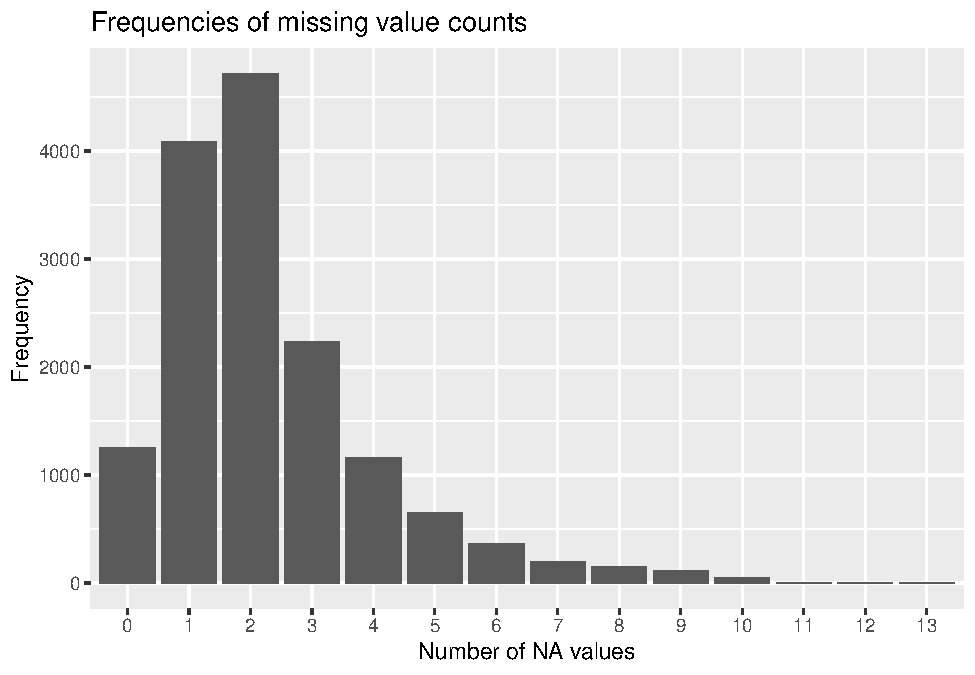
\includegraphics{hw2_files/figure-latex/unnamed-chunk-5-1.pdf}

\begin{enumerate}
\def\labelenumi{\arabic{enumi}.}
\setcounter{enumi}{1}
\tightlist
\item
  The regression lines of all the plots are very similar if not
  identical. All the lines have a slight negative slope. However, the
  actual points of each dataset are completely different from each
  other. The very similar statistical summaries masks this.
\end{enumerate}

\end{document}
